\documentclass[tikz]{standalone}
\usetikzlibrary{automata,positioning}

\usepackage[T1]{fontenc}
\usepackage[familydefault,regular]{Chivo}
\usepackage{xcolor}

\definecolor{900}{HTML}{B71C1C}

\begin{document}
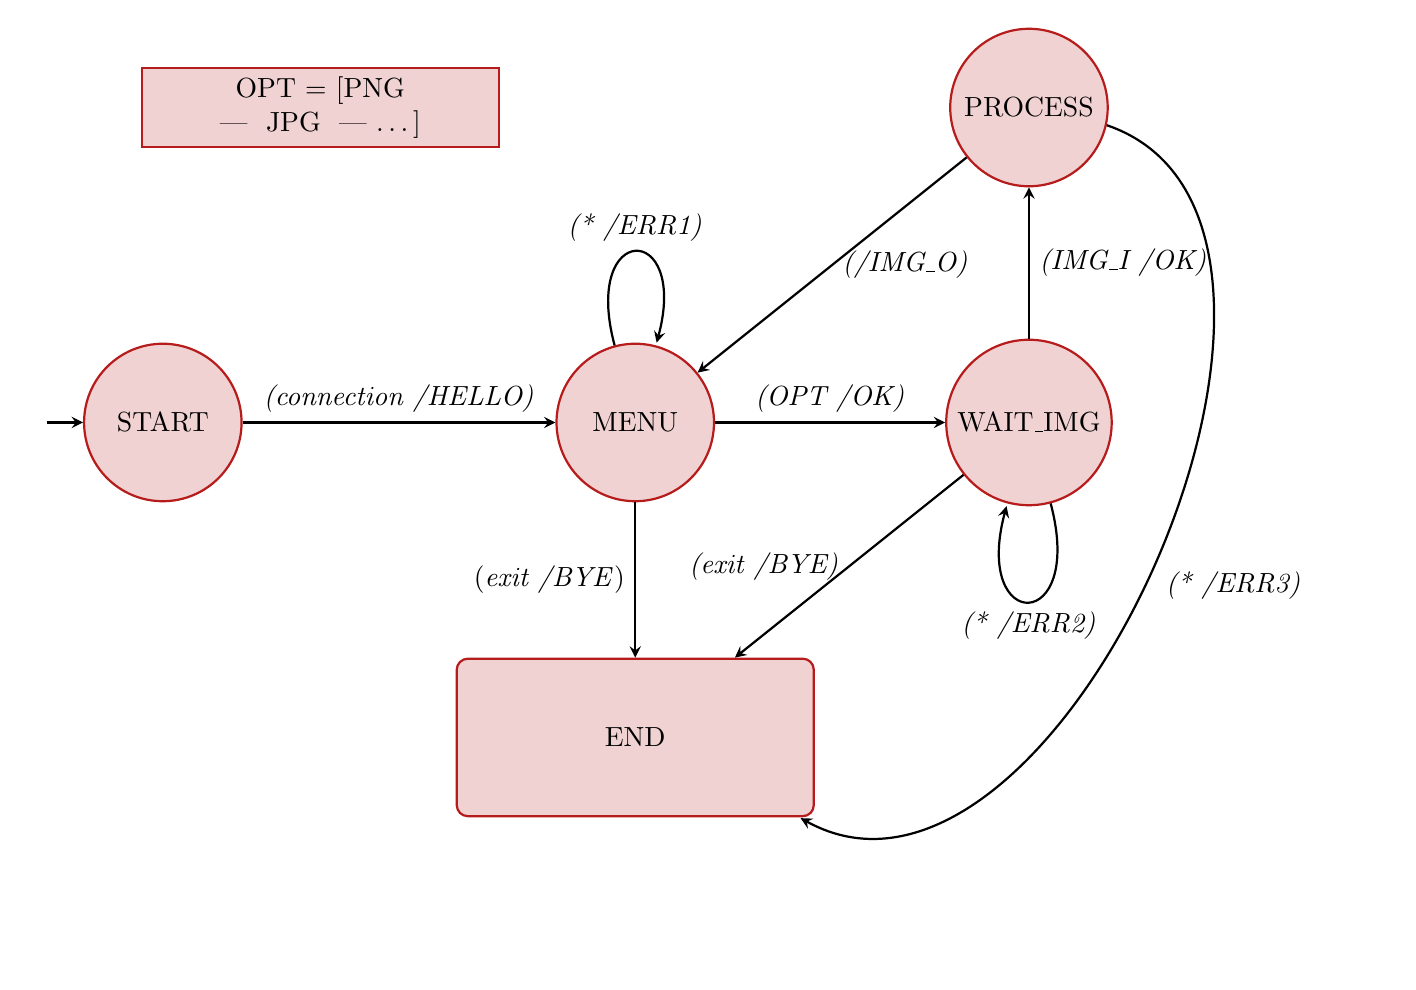
\begin{tikzpicture}[>=stealth,node distance=4cm,on grid,auto, thick, initial text=]
\tikzstyle{state}=[circle,thick,draw=900,fill=900!20,minimum size=20mm]
\tikzstyle{key}=[rectangle, draw=900, fill=900!20, text=black, text centered, text width=43mm]

	\node[state,initial] 	(q_0)	{START};
	    \node[key] (key) [above right =4cm and 2cm of q_0] {OPT = [PNG \ | \ JPG \ | \dots]};
	\node[state]		 	(q_1) [right=6cm of q_0]	{MENU};
	\node[state]	        (q_2) [right=5cm of q_1]	{WAIT{\_}IMG};
	\node[state]			(q_3) [above= of q_2]	{PROCESS};
	\node[state]			(q_7) [below=of q_1]	[text width=43mm,rectangle, rounded corners, text centered]{END};
	
	\path[->]	(q_0) edge node[above] [align=center] {\textit{(connection /HELLO)}} (q_1)
				(q_1) edge node[above] {\textit{(OPT /OK)}} (q_2)
				      edge [loop above] node {\textit{(* /ERR1)}} (q_1)
				      edge node[left] {(\textit{exit /BYE})} (q_7)
				(q_2) edge [left] node[right] {\textit{(IMG\_I /OK)}}   (q_3)
				      edge [loop below] node {\textit{(* /ERR2)}} (q_2)
				      edge node[left] {\textit{(exit /BYE)}} (q_7)
				(q_3) edge [left] node[right] {\textit{(/IMG\_O)}}   (q_1)
				      edge [bend left=95] node {\textit{(* /ERR3)}} +(-2.9,-9.025);
\end{tikzpicture}
\end{document}